

\section{3. MECAGEN Biomechanics  }   ...
\\ ...
\\ ...
\\ ...
\\ ...
\\ ...
\\ ...
\\ ...
\\ ...
\\ ...
\\ ...
\\ ...
\\ ...
\\ ...
\\ ...
\\ ...
\\ ...
\\ ...
\\ ...
\\ ...
\\ ...
\\ ...
\\ ...
\\ ...
\\ ...
\\ ...
\\ ...
\\ ...
\\ ...
\\ ...
\\ ...
\\ ...
\\ ...
\\ ...
\\ ...
\\ ...
\\ ...
\\ ...
\\ ...
\\ ...
\\ ...
\\ ...
\\ ...
\\ ...
\\ ...
\\ ...
\\ ...
\\ ...
\\ ...
\\ ...
\\

\subsection{3.1. State of the Art  }   ...
\\ ...
\\ ...
\\ ...
\\ ...
\\ ...
\\ ...
\\ ...
\\ ...
\\ ...
\\ ...
\\ ...
\\ ...
\\ ...
\\ ...
\\ ...
\\ ...
\\ ...
\\ ...
\\ ...
\\ ...
\\ ...
\\ ...
\\ ...
\\ ...
\\ ...
\\ ...
\\ ...
\\ ...
\\ ...
\\ ...
\\ ...
\\ ...
\\ ...
\\ ...
\\ ...
\\ ...
\\ ...
\\ ...
\\ ...
\\ ...
\\ ...
\\ ...
\\ ...
\\ ...
\\ ...
\\ ...
\\ ...
\\ ...
\\ ...
\\

\subsubsection{3.1.1. Soft material no physics available  }   ...
\\ ...
\\ ...
\\ ...
\\ ...
\\ ...
\\ ...
\\ ...
\\ ...
\\ ...
\\ ...
\\ ...
\\ ...
\\ ...
\\ ...
\\ ...
\\ ...
\\ ...
\\ ...
\\ ...
\\ ...
\\ ...
\\ ...
\\ ...
\\ ...
\\ ...
\\ ...
\\ ...
\\ ...
\\ ...
\\ ...
\\ ...
\\ ...
\\ ...
\\ ...
\\ ...
\\ ...
\\ ...
\\ ...
\\ ...
\\ ...
\\ ...
\\ ...
\\ ...
\\ ...
\\ ...
\\ ...
\\ ...
\\ ...
\\ ...
\\

\subsubsection{3.1.2. Classical mechanics versus statistical mechanics  }   ...
\\ ...
\\ ...
\\ ...
\\ ...
\\ ...
\\ ...
\\ ...
\\ ...
\\ ...
\\ ...
\\ ...
\\ ...
\\ ...
\\ ...
\\ ...
\\ ...
\\ ...
\\ ...
\\ ...
\\ ...
\\ ...
\\ ...
\\ ...
\\ ...
\\ ...
\\ ...
\\ ...
\\ ...
\\ ...
\\ ...
\\ ...
\\ ...
\\ ...
\\ ...
\\ ...
\\ ...
\\ ...
\\ ...
\\ ...
\\ ...
\\ ...
\\ ...
\\ ...
\\ ...
\\ ...
\\ ...
\\ ...
\\ ...
\\ ...
\\

\subsubsection{3.1.3. Particle-based physics  }   ...
\\ ...
\\ ...
\\ ...
\\ ...
\\ ...
\\ ...
\\ ...
\\ ...
\\ ...
\\ ...
\\ ...
\\ ...
\\ ...
\\ ...
\\ ...
\\ ...
\\ ...
\\ ...
\\ ...
\\ ...
\\ ...
\\ ...
\\ ...
\\ ...
\\ ...
\\ ...
\\ ...
\\ ...
\\ ...
\\ ...
\\ ...
\\ ...
\\ ...
\\ ...
\\ ...
\\ ...
\\ ...
\\ ...
\\ ...
\\ ...
\\ ...
\\ ...
\\ ...
\\ ...
\\ ...
\\ ...
\\ ...
\\ ...
\\ ...
\\

\subsection{3.2. Hypotheses  }   ...
\\ ...
\\ ...
\\ ...
\\ ...
\\ ...
\\ ...
\\ ...
\\ ...
\\ ...
\\ ...
\\ ...
\\ ...
\\ ...
\\ ...
\\ ...
\\ ...
\\ ...
\\ ...
\\ ...
\\ ...
\\ ...
\\ ...
\\ ...
\\ ...
\\ ...
\\ ...
\\ ...
\\ ...
\\ ...
\\ ...
\\ ...
\\ ...
\\ ...
\\ ...
\\ ...
\\ ...
\\ ...
\\ ...
\\ ...
\\ ...
\\ ...
\\ ...
\\ ...
\\ ...
\\ ...
\\ ...
\\ ...
\\ ...
\\ ...
\\

\subsubsection{3.2.1. Equation of Motion  }

Newton's second law states that the acceleration $\vec{a}$ of a body is proportional to the sum of the forces applied to it $\vec{F}$. The proportionality factor is the inverse of the mass of the body, a quantity assumed to remain constant over time.

$$ m \vec{a} = \vec{F} $$

In particle-based physics, each particle $p_i$ (mass $m_i$, position $X_i$, velocity $v_i$, acceleration $a_i$, size $R_i$) are related by the Newton's law straightforwardly:

$$m_i \vec{a_i} = \vec{F}(X_i, v_i, R_i, ...)$$

However, the physical world in which cells evolve is a very counterintuitive one. Cells are so small and their interaction are so sticky that the physics of their motion is radically different from the one we are accustomed to. The main difference is the disappearance of inertial forces.

In “Life at low Reynolds number” (see Purcell, Life at low Reynolds number. American Journal of Physics (1977)), E.M. Purcell explains how a water-immersed cell stops moving as soon as he stops pushing it. The cell, an E. Coli bacteria, is so small that the viscous forces exerted by the surrounding water are overwhelming the inertial forces due to the motion. 

When an object of characteristic length $R$ moves at a velocity $v$ in a fluid of density $\rho$ and dynamic viscosity $\mu$, the quantity that measures the ratio of the inertial forces to the viscous forces is called the Reynolds number $Re$. This dimension-less number is expressed as the following:

$$Re = \frac{\rho v R}{\mu}$$

The ratio $\frac{\mu}{\rho}$ is the kinematic viscosity $\nu$ and it has a value of $ 10^{-6} {m}^2 {s}^{-1} $  for water.

For a man of characteristic length $1m$ swimming at $1 m s^{-1}$, $Re$ is about $10^6$. For a bacterium of characteristic length $10^{-6} m$ swimming at $10^{-5} m s^{-1}$, $Re$ is $10^{-5}$. The physics of inertia and viscosity is totally different for these two examples. The balance shifts from inertial forces for a man to the viscosity forces for a cell.

A more striking example is the coasting distance of the same bacterium when it stops self-propulsing in water. When only inertial and viscous and inertial are at work, Newton's second law is written:

$$m \frac{dv}{dt} = - \gamma_{drag} v$$

The solution is $v(t) = v_0 e^{ -\frac{\gamma_{drag}}{m} t}$ (see Introductory Biophysics - Perspectives on the living state p.96 by J. Claycomb and J. Tran)

Integrating it from $t=0$ to $t=\inf$, gives the coasting distance of the bacterium $d$:

$$d = \frac{v_0 m}{\gamma_{drag}}$$

For a bacterium swimming at $10^{-5} m s^{-1}$, this distance is $0.1$ angstrom.

This simple calculus confirms that if the bacterium is not moving by itself or pushed by an external actor, it stops “immediatly” its motion.

Purcell interprets theses results as the following: “If you are at very low Reynolds number, what you are doing at the moment is entirely determined by the forces that are exerted on you \underline{at the moment}, and by nothing in the past.”

This implies that in these low Reynolds environments, applied forces produce a velocity, not an acceleration. The displacement is proportional the instantaneous force and inversely proportional to the a damping coefficient $\lambda$

Theses results thereby allow a bypass of Newton's Second Law and we write the new equation of motion that will be used in our model :

$$\lambda \vec{v} = \vec{F}$$

The previous argument has been evaluated for a solid object moving in a fluid flow. In a multicellular environment as encountered in developing systems, we assume that the aforementioned principle remains the same because:
\begin{itemize}
	\item the dimension of the cells are similar to the aforementioned bacterium (from 300 microns for the zygote to 0.3 microns at stage 1024 cells, 0.02 microns when the embryo is composed of about 15000 cells), 
	\item the density is equivalent.
	\item the kinematic viscosity of the surrounding cells taken as a flow can be considered greater than the one of water. For example, at 18°C, the kinematic viscosity of ketchup is 50000 times higher than the one of water. (see Odell et al. The mechanical basis of morphogenesis. I. Epithelial folding and invagination. Developmental Biology (1981) Appendix 2 for a similar justification)
\end{itemize}

For each particle $p_i$, its motion is governed by its interactions with neighbor cells:

$$\lambda_i \vec{v}_{i} = \sum_{neighbors\;j} \vec{F}_{i,j}$$

The main difference with the example of a solid object is that the surrounding cells are responsible for the damping of the motion but also for the motion itself. Here there is no hand pushing the cell like Purcell explained, the pushing is executed by every cell intrinsic behavior. 

This is why these interactions are decoupled in the following way:
\begin{itemize}
	\item the damping coefficient $\lambda$ assure the global damping of the particle. (It plays an equivalent role as the mass in Newton's Second Law). This weighting coefficient is proportional to the inverse of the surface of the cell: $ \lambda_i = \lambda_0 {R_i}^2$ (show study of R^0, R^1, R^2). 
	\item A passive force $\vec{F_P}$ of interaction between neighbor cell maintains the integrity of the cellular volume and controls both the stiffness and the adhesion of their interaction. This force is always exerting its action whatever the state of the cell. However, it is modulated through its stiffness and adhesion. 
	\item An active force $\vec{F_A}$ of interaction between neighbor cell executes specific behavior like protrusive activity or apical constriction. The force depends of the state of the cell and it disappears when the cell is in a “resting” state.
\end{itemize}

The weight, exerted by earth gravitational field, derived from Newton's law of universal gravitation $W_i = m_i \frac{G  M_{earth}}  {{R_{earth}}^2} $ is neglected. 

$$\vec{v}_{i} =  \frac{1}{\lambda_i} \sum_{neighbors\;j} \left ( \vec{F_P}_{i,j} + \vec{F_A}_{i,j} \right )$$    ...
\\ ...
\\ ...
\\

\subsubsection{3.2.2. Spatial Neighborhood  }

Cell sustains forces from the cells which are in contact with them. The notion of contact is straightforward in some modeling paradigm (potts for example) but in highly abstracted model like particle-based model, specific algorithm are to be devised. 

At each time step, the only information about the spatial structure is that each cell, represented by a spheroidal particle $p_i$ belonging to a swarm $S$, has a position $X_i (x_i,y_i,z_i)$, and of volume $V_i$ (see fig below left). The objective of this part is to infer the neighboring links and contact surface area as in fig XX.

The regular Delaunay triangulation is in many way the most adapted method, it establishes a list of neighbors according to topological criteria dependent of each particle size (see state of the art). However, its drawback is its computational heaviness. We have adopted a parallel algorithmic structure exploiting the computational power of GPGPU (see relevant part), and, to our knowledge, there is no parallel implementation for regular triangulation yet.

We designed a new parallel neighboring building strategy (see algorithm part for implementation) which insure that a topologically plausible structure is realized.

A comparison between the regular triangulation and our neighboring strategy is proposed at the end of this part.

Our method consecutively builds two lists of neighbor particles. The first selection $\mathcal{N}_m (p_i)$, based on metric criteria, is filtered by a topological criteria to define the final selection of neighbors $\mathcal{N}_t (p_i)$.

\textbf{Metric selection of neighbor particles}

Two cells of radius $R_i$, $R_j$ and of position $X_i$ and $X_j$ are considered neighbor according to the metric criteria iff their relative distance is less than a constant factor $c_{max}$ times the sum of their radii $R_i+R_j$.

We denote by $r_{max}$ this cutoff value: $r_{max} = c_{max} (R_i+R_j)$.

The set of neighbor particle of a particle $p_i$ according to the metric criteria is defined by the following:

$$\mathcal{N}_m (p_i) := \left \{  p_j \in S : \left \|  X_i - X_j \right \| \leq c_{max} \cdot (R_i+R_j) \right \} $$

Even if the particles are considered "spheroidal", we incorporate the ability to deform to access farer neighbor cells. $r_{max}$ sets the maximum distance of this deformation. The sphere of radius $r_{max}$ represents the domain of space where the particle can potentially interact.

More generally, we need to define a law that relates the distance between two neighbor particles to the area of the contact surface. $r_{max}$ is the limit from which this area is equal to zero.

\textbf{Empirical quantification of the surface of contact}

In the absence of real experimental data, we generate an artificial construction based on the weighted delaunay triangulation. This will allow us to infer an empirical law which approximate the surface-distance relationship in this articifial case and, by extension, to the modeled multicellular system.

An ellipsoidal domain of space is filled with particles belonging to three consecutive cell generation $g1$, $g2$, $g3$ in equal proportion. Their volume are /(V_{g1}/), /(V_{g2}=  \frac{1}{2} V_{g1}/), $V_{g3} = \left ( \frac{1}{2} \right )^{2} V_{g1}$. Similarly, the particle being considered spheroidal, their radii are $R_{g1}$, $R_{g2} = \left ( \frac{1}{2} \right )^{\frac{1}{3}} R_{g1}$, $R_{g3} = \left ( \frac{1}{2} \right )^{\frac{2}{3}} R_{g1}$. These radii are the weighing coefficient of the triangulation.

The number $N$ of each particle generation is determined to fit the total volume occupied by the $3N$ particles with the volume of the ellipsoid.

The ellipsoid self deforms to impose a rearrangement of the particles, generating various spatial reorganisation. The first semi-principal axis of the ellipsoid is cycling sinusoidallly, the second remains constant and the third is specified to maintain the volume of the ellipsoid constant.
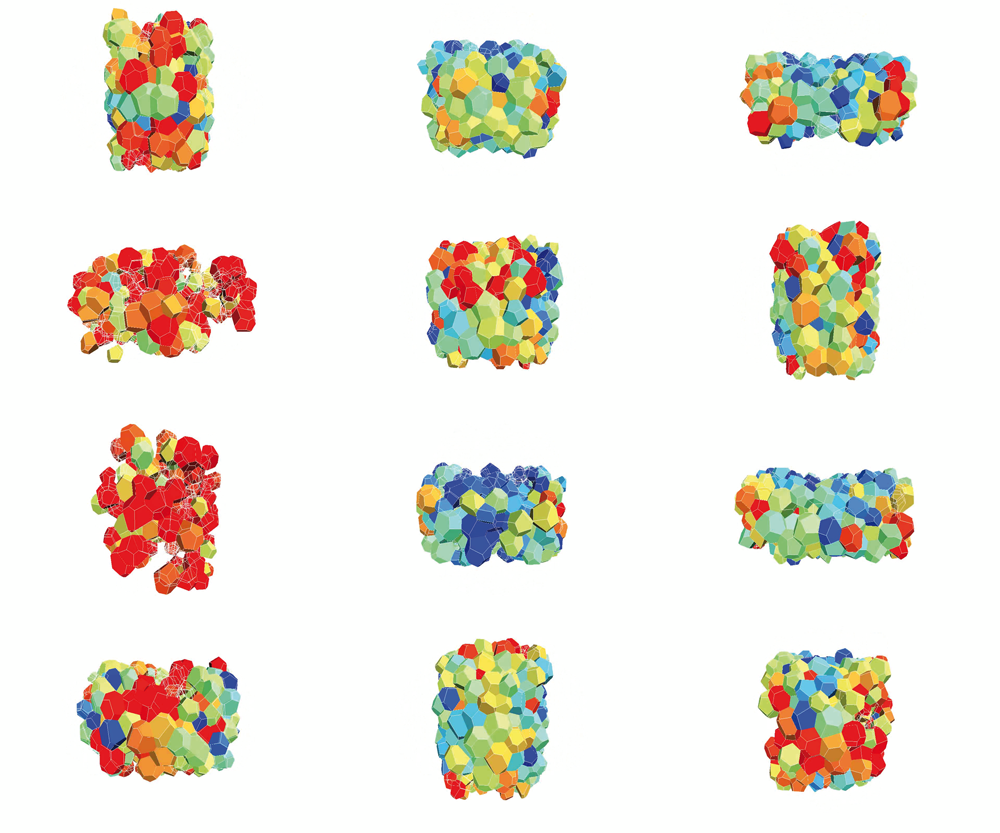
\includegraphics{../../images/MECAGEN/spatial_neighb/surf_dist_movie_1677cells_gS11_filtered_SNAPSHOT/Fusion_light.png}

On the figure above, only the close Voronoï volume that does not belong to the convex hull are shown. The color code highlights the normalized difference of volume between the theoretical volume of the cell and the volume specified by the weighted Voronoï $c = \frac{V_{obs} - V_{theo}}{V_{theo}}$. 

When two neighbor cells both have a measure $c$ which is less than 5% (green cell in figure XX), we consider that these cells have a valid spatial configuration and we store the pair composed of their relative distance and the area of the surface of contact ie the area of the Voronoï face shared by both cell.

We will denote by an experiment $i$ the aforementioned simulation with a set of $N$ particle of generation $g1=i$, $g2=i+1$ and $g3=i+2$. Each experiment thereby creates 6 sets of data called plots: a plot for every possible pair of generation ($g1/g1, g1/g2, g1/g3, g2/g2, g2/g3, g3/g3$).

We performed 6 experiments with $i$ belonging to the set $\left [ 9, 14 \right ]$. Theses generations correspond to the zebrafish generations which can be mixed. It explains why the indices start at 9 but this fact is not relevant for the following study. 
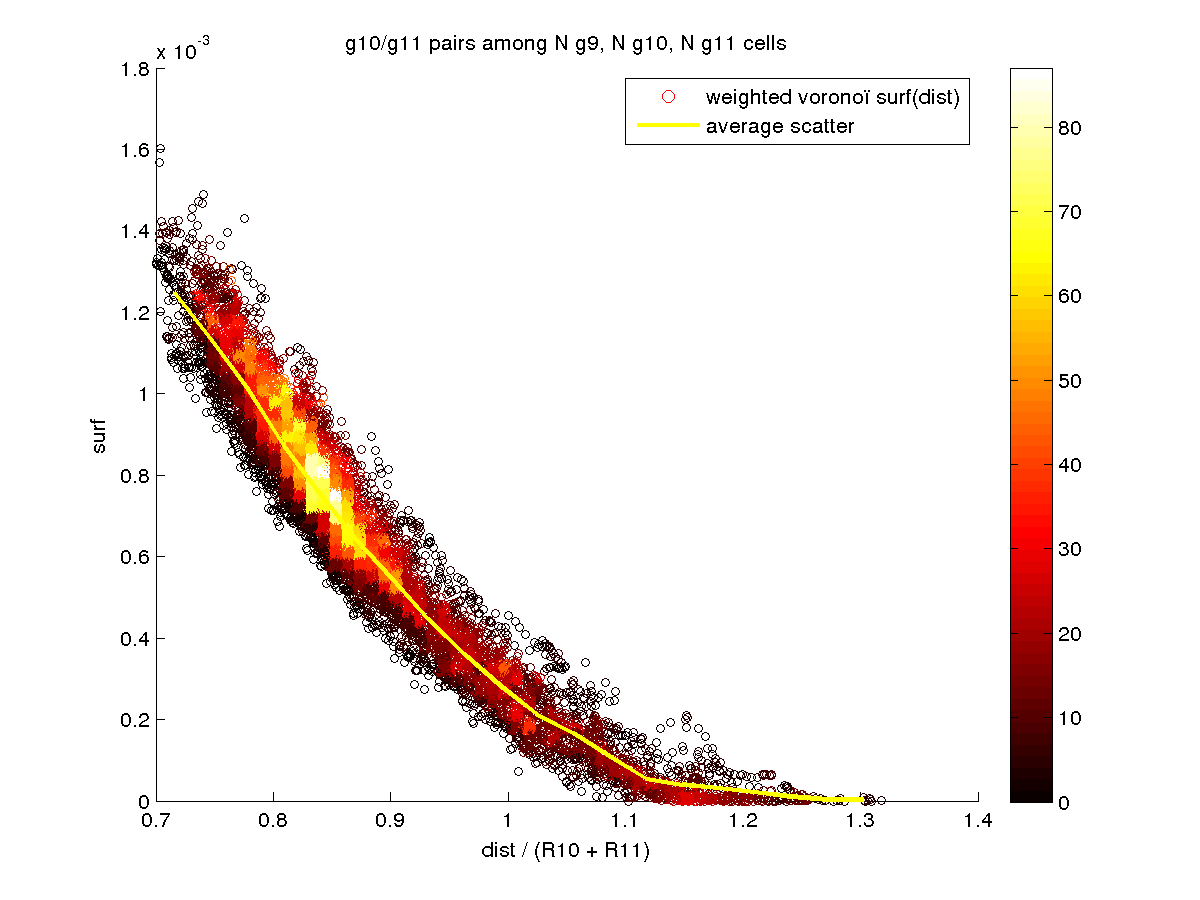
\includegraphics{../../images/MECAGEN/spatial_neighb/g10_g11_exp9_simple.png}

For each plot, $numPoints(exp,g1,g2)$ points $\left ( dist_{exp,g1,g2}(i), surf_{exp,g1,g2}(i)  \right ), i \in \left [ 1,numPoints(exp,g1,g2) \right ]$ are collected, typically about 10000. We observe that, as expected, if most points are located below the distance $R_i+R_j$, some of them exceed it.

The selected empirical law is written:

$$ A(r,R_i,R_j) = \begin{cases}  a (r - c_{max} (R_i+R_j))^2 & \text{if }r< r_{max} (R_i+R_j) \\ 0 & \text{if }r\geq r_{max}(R_i+R_j)  \end{cases}$$

We decide to use a monomial of degree 2 in order to scale as a surface. If the distance $r$ between two double-sized neighbor particles $p_i$ and $p_j$ is doubled, the area of the surface of contact will quadruple.

$$A(2r,2R_i,2R_j) = 4 A(r,R_i,R_j)$$

To obtain the best pair of parameters $(a, c_{max})$, the discrepancy between the generated data and the empirical law is measured with the "sum of squared errors of prediction" (SSE) function. The smaller the SSE is, the better the law matches the data.

In general terms, the SSE is expressed: 

$$SSE = \sum_{i = 1}^{n} \left ( y_i - f(x_i) \right )^2$$

In our case, the sample of variable is split in 6 experiments and 6 couple of particle types ($g1/g2$) per experiment, the ith observed variable $y_i$ is the measured area of surface of contact $surf_{exp,g1,g2}(i)$, and the value of the predicted variable $f(x_i)$ is the value of the empirical law at the observated variable distance $A(dist_{exp,g1,g2}(i),R_{g1},R_{g2})$. The SSE is written:

$$SSE (a,r_{max}) = \sum_{exp = 9}^{14} \sum_{g1 = exp}^{exp+2} \sum_{g2 = g1}^{exp+2} \left ( \frac{1}{< surf_{exp,g1,g2}>} \sum_{i = 1}^{numPoints(exp,g1,g2)}  \left ( surf_{exp,g1,g2}(i) - a(dist_{exp,g1,g2}(i) - c_{max} (R_{g1} + R_{g2})) \right )^2 \right )$$

We explored exhaustively all the couple $(a,c_{max})$ until the 4th decimal. A heatmap of this exploration is vizualised below.
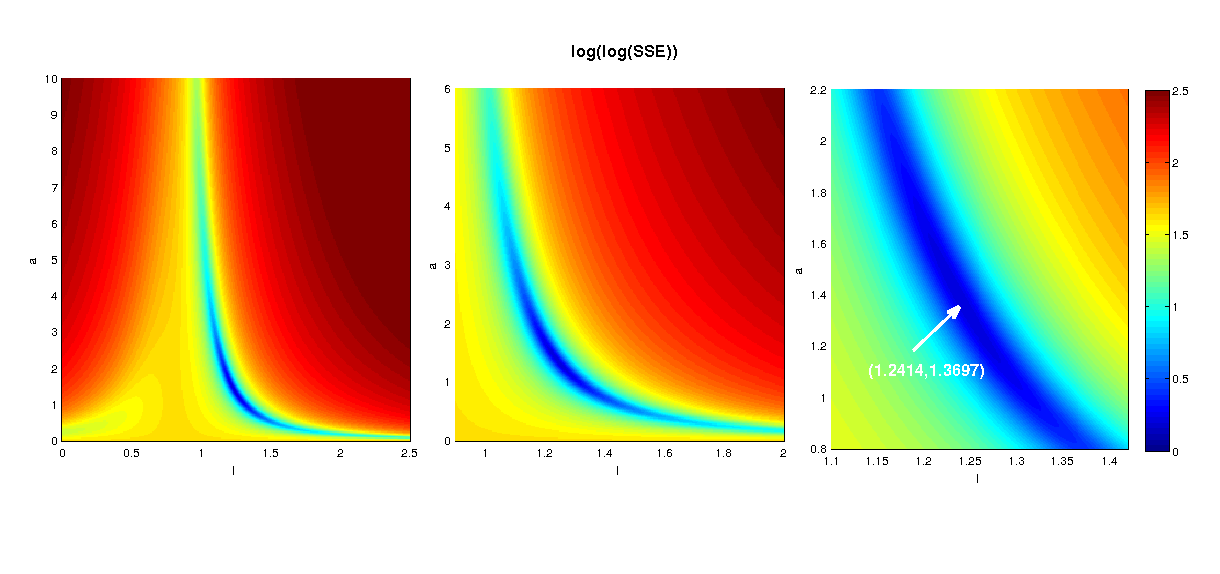
\includegraphics{../../images/MECAGEN/spatial_neighb/zoomALL.png}

The best couple with four decimal is $(a=1.3697 , c_{max}=1.2414)$. These values are used throughout the rest of the manuscript.

To compare the empirical law with the generated data, the following figure proposes an overlay of both data on 6 plots.
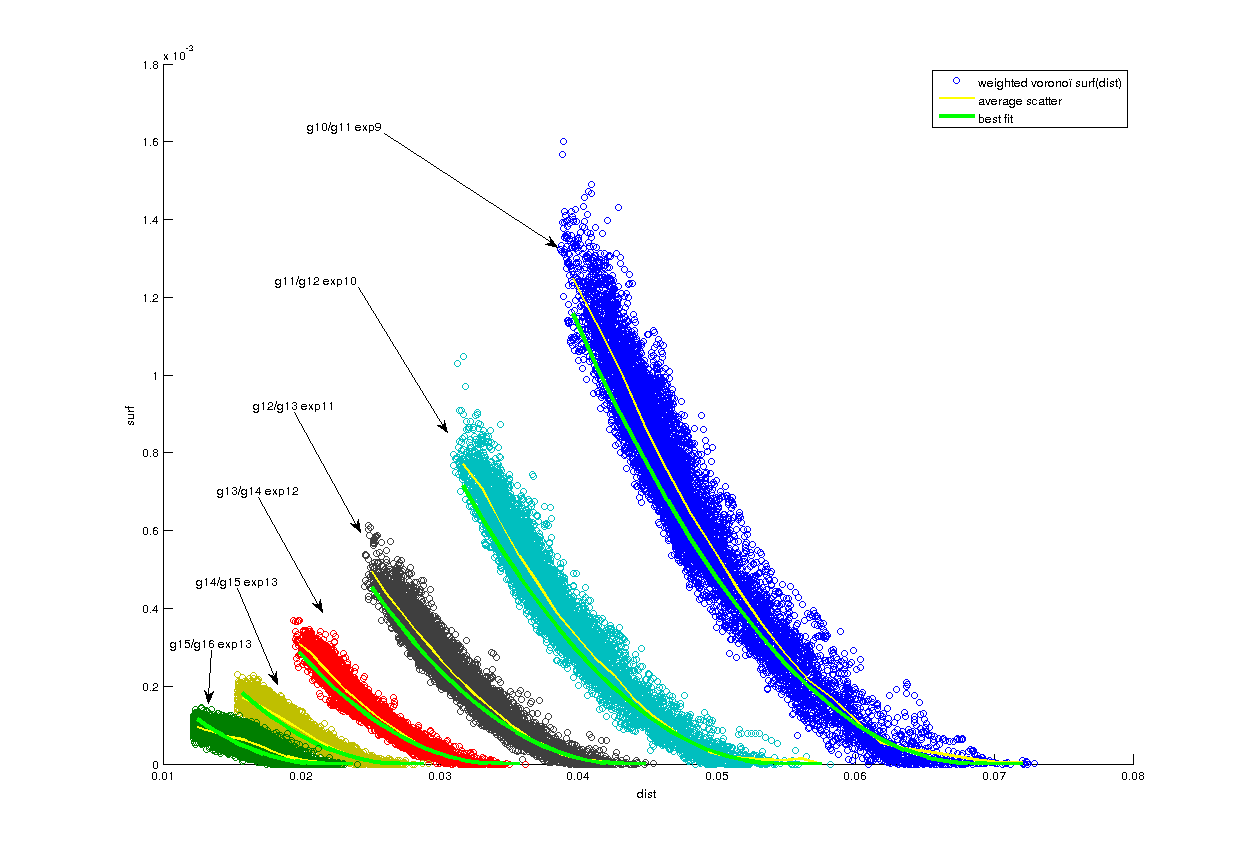
\includegraphics{../../images/MECAGEN/spatial_neighb/multi_scatter_gp1_gp2_exp9_14.png}

\textbf{Topological selection of neighbor particles}

As exposed in the state of the art, a metric neighboring selection is not sufficient as it leads to collapsing simulation for high adhesive particle interactions. We propose to use a filtering of the metric list of neighbor with a topological criteria to avoid this drawback.

The delaunay triangulation solve this issue but is slow to compute because of its heavy data structure composed of tetraedra. Our solution is inspired by a similar neighboring method: the Gabriel graph.

In 2D, where the Delaunay triangulation imposes that no particle is inside the circumcircle of any triangle of the Delaunay triangulation, the Gabriel graph method imposes that no particle lie inside the circle whom diameter is a valid neighboring link.
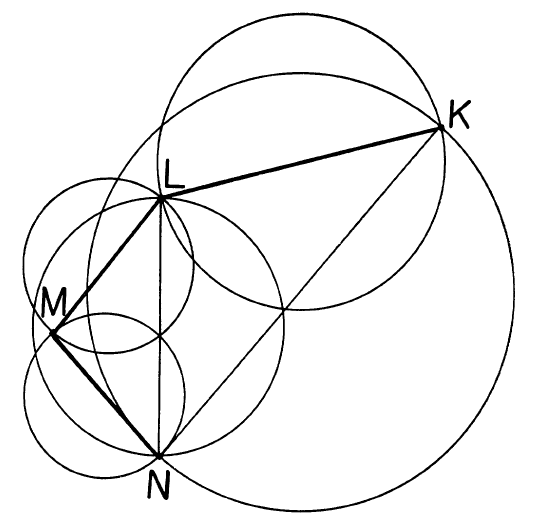
\includegraphics{../../images/MECAGEN/spatial_neighb/gabriel.png}Gabriel graph as introduced in Gabriel and Sokal. A new statistical approach to geographic variation analysis. Systematic Biology (1969)

We propose to extend the method in the 3D case: each particle pair $(p_i, p_j)$ is considered valid according to the Gabriel criteria if no other particle of the swarm lie inside the ball whose diameter is $\left [ X_i X_j \right ] $.  *********** 

 Note de bas de page:  To our knowledge, the term Gabriel graph has not been formally defined in 3D. However, when it is mentionned (see Attali and Montanvert. Computing and simplifying 2D and 3D continuous skeletons. Computer Vision and Image Understanding (1997)), a 3D version of the Gabriel graph does not use an edge to define the empty ball criteria but a triangle. This makes sense, in n-dimension, Delaunay triangulation uses n-simplices as basic units for defining the empty ball criteria ie a triangle in 2D and tetrahedron in 3D. In 2D, the Gabriel graph uses a (n-1)-simplex as a basic unit (an edge), the straightforward equivalent in 3D would also use a (n-1)-simplex ie a triangle. Yet for the sake of clarity, we will still denote the edge defining the empty ball criteria by Gabriel. (ou pas ? René? Une idée de nouveau nom??) fin note de bas de page ***************   

Two cells of radius $R_i$, $R_j$ and of position $X_i$ and $X_j$ are considered neighbor according to the topological criteria iff no neighbor cell according to the metric criteria have their position inside the sphere of diameter $[X_i X_j]$.

$$\mathcal{N}_t (p_i) := \left \{  p_j \in  \mathcal{N}_m (p_i) : \forall p_k \in  \mathcal{N}_m (p_i), \left \| \frac{1}{2} ( X_i + X_j ) - X_k  \right \| \geq \frac{1}{2} \left \| X_i - X_j \right \|\right \} $$

In fact, in the 2D case, the Gabriel graph is a subgraph of the Delaunay triangulation. Every pair of neighbor in a Gabriel graph are also neighbor according to the Delaunay criteria (see figure XX). 
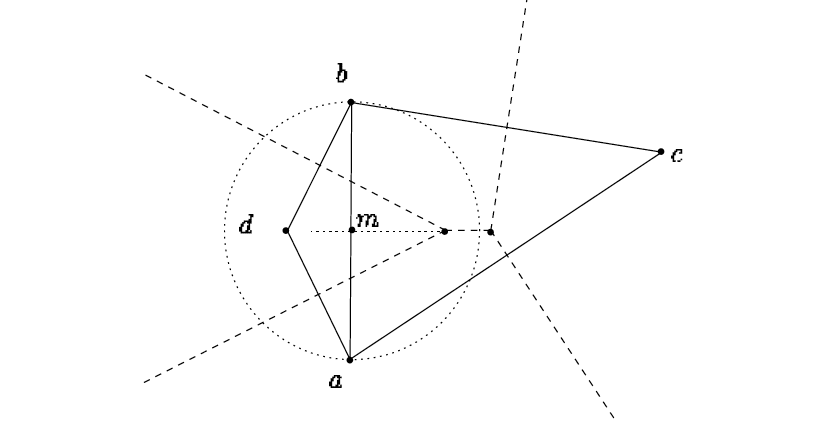
\includegraphics{../../images/MECAGEN/spatial_neighb/gabdelau.png}The solid edges materialize neighborhood according to the Delaunay triangulation, all edges but edge ab are Gabriel edges. A visual way to determine if a Delaunay edge is also a Gabriel edge is to check if the edge crosses the surface of contact (here edge of contact). If the Delaunay edge pass through it, it is also a Gabriel edge. The edge we loose with our approximation are the one which matter the less. Picture from Cazals and Giesen. Delaunay Triangulation Based Surface Reconstruction : Ideas and Algorithms. (2004)

TODO: plot the ratio of gabriel edges which are also delaunay edges in Mecagen. To confirm the validity of our hypethesis.

\subsubsection{3.2.3. Interaction Potential  }

Two neighbor spheroidal particles with radii $R_i$ and $R_j$, separated with by a distance $r$, will interact by means of forces $ \vec{F}_{i,j} $. In MECAGEN, these forces are decomposed in two parts: 
\begin{itemize}
	\item Relaxing forces, derived from an attraction/repulsion potential. They relax the swarm of particles toward an equilibrium state. The underlying principle is the surface maximization of every neighbor pair in the swarm.
	\item Behavioral forces which move the swarm configuration away from the previous equilibrium. These behavior are inspired by the protrusive activity of the cell.
\end{itemize}

Every pair of neighbor particles interaction potential share common features: repulsion at short distance, until an equilibrium distance $c_{eq} (R_i+R_j)$ and attraction afterwards, until the limit of the interaction field $r_{max} $. We already discussed how MECAGEN deals with the limit, we will present now how is determined the equilibrium distance.

\textbf{Distance of equilibrium}

With respect to the observation that equilibrium distance which depends on biomechanical parameters does not have a solid theoretical foundation in multicellular systems (see state of the art), we decide that the distance equilibrium of neighbor cells corresponds to the distance between center in the densest arrangement of sphere pack. We assume that there is no significant volume is occupied by intercellular material. Otherwise, additional particle representing the extra-cellular material should be added (not presented here).

On a 2D plane, the densest arrangement of all possible circle packing is the hexagonal lattice (see figure XX). The ratio of the surface occupied by the disks to the surface containing the disks is equal to the ratio of the surface of a disk to the surface of an hexagon i.e. $\frac{\pi}{ 2 \sqrt{3}} \simeq 0.9068997...$.

In 3D, Kepler conjecture states that the hexagonal close packing and face-centered cubic close packing arrangements of equally sized sphere have the greater density of all arrangement (proven by Thomas Hales in 1998). An hexagonal close packing arrangement is obtained by superposing alternatively two 2D hexagonal lattice of sphere with pattern ABAB... (see figure XX).

In this arrangement, each sphere touches 12 other spheres ie each particle has 12 neighbors (six particles on a 2D plane and three other particles on each of the surrounding planes). The space-filling tessellation which is dual to this arrangement has a tile called trapezo-rhombic dodecahedron (TRD) (see figure XX).
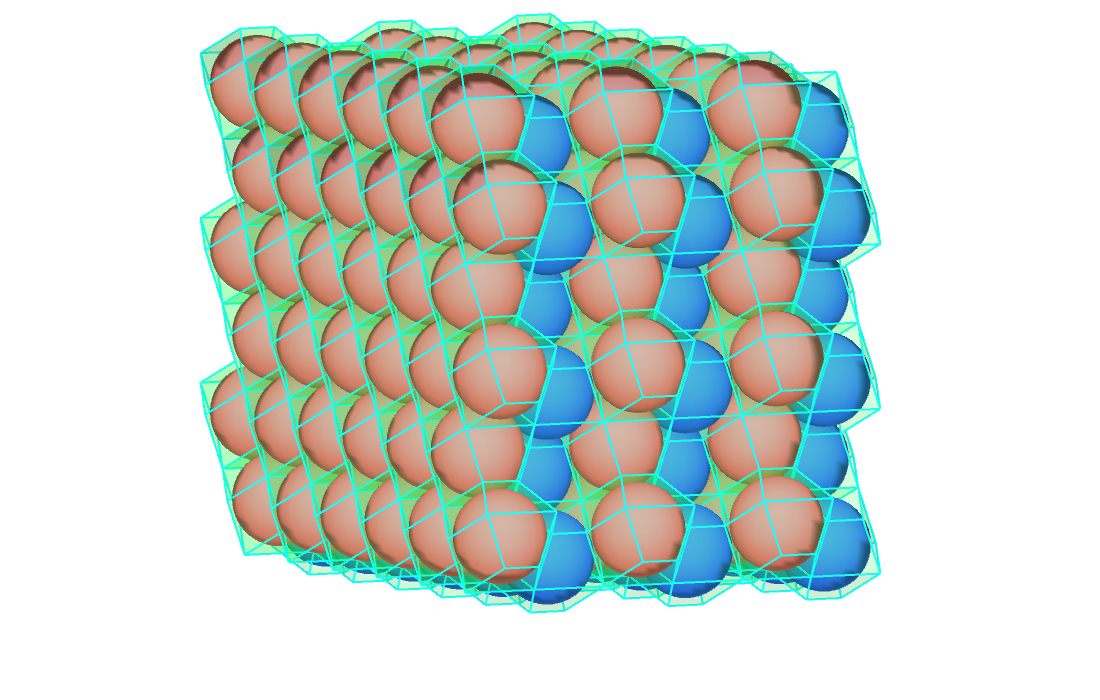
\includegraphics{../../images/MECAGEN/potential/trapezo_swarm.png}
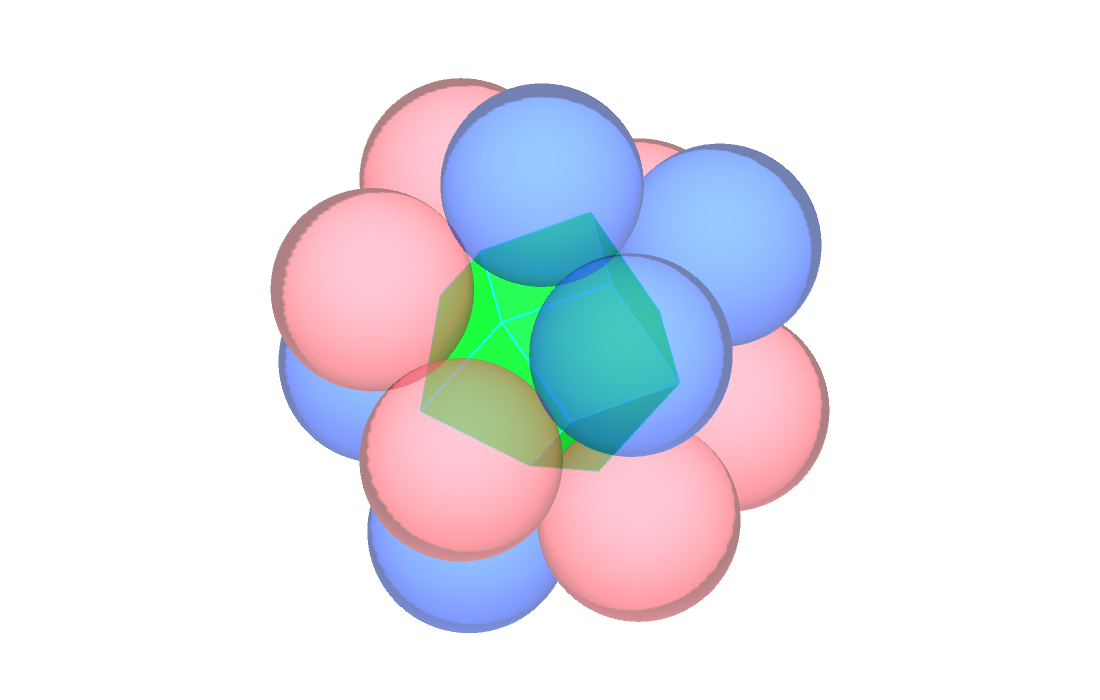
\includegraphics{../../images/MECAGEN/potential/trapezorhombicdodecahedron.png}

The atomic packing factor is the ratio of the volume of a sphere to the volume of the TDR and it is equal to $\frac{\pi}{3\sqrt{2}} \simeq 0.74048... $. So, for a pair of cells of radii $R_i = R_j=R$, their equilibrium distance is:

$ r_{eq} = {\frac{\pi}{3\sqrt{2}}} ^ {1/3} \left ( R_i + R_j \right ) $, with $c_{eq} = {\frac{\pi}{3\sqrt{2}}} ^ {1/3} \simeq 0.904699895...$ 

We extend the notion of distance of equilibrium in a pair of neighbor particle to the notion of a radius of equilibrium intrinsic to the particle. It means that each particle brings its own contribution to equilibrium distance between two neighbor cells.   

We denote by $r_{eq}(p_i)$ the radius of equilibrium of the particle $p_i$. $r_{eq}(p_i) = c_{eq}R_i$ (see figure XX)

In a pair of neighbor particle $p_i$, $p_j$, we get:

$$ r_{eq} = r_{eq}(p_i) + r_{eq}(p_j) $$
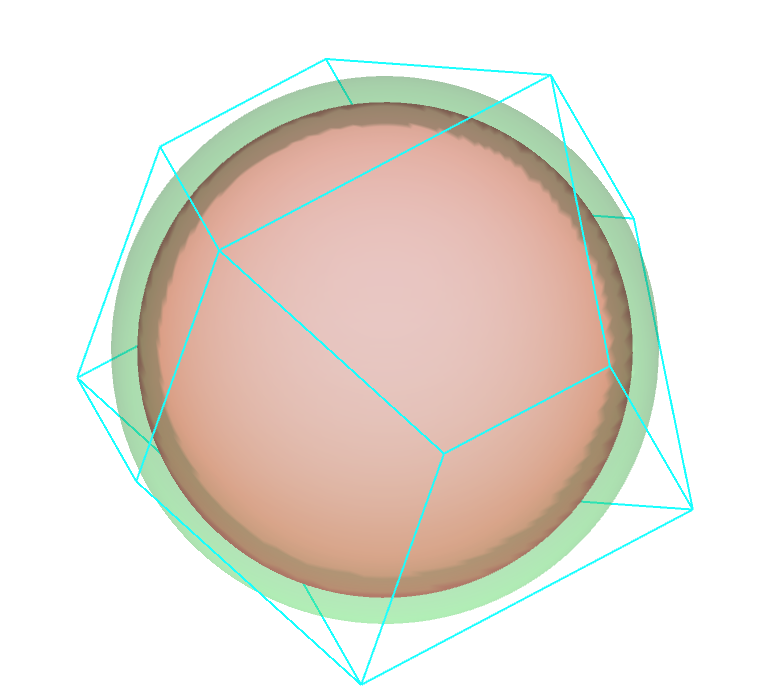
\includegraphics{../../images/MECAGEN/potential/apf_sphere_raw2_crop.png}
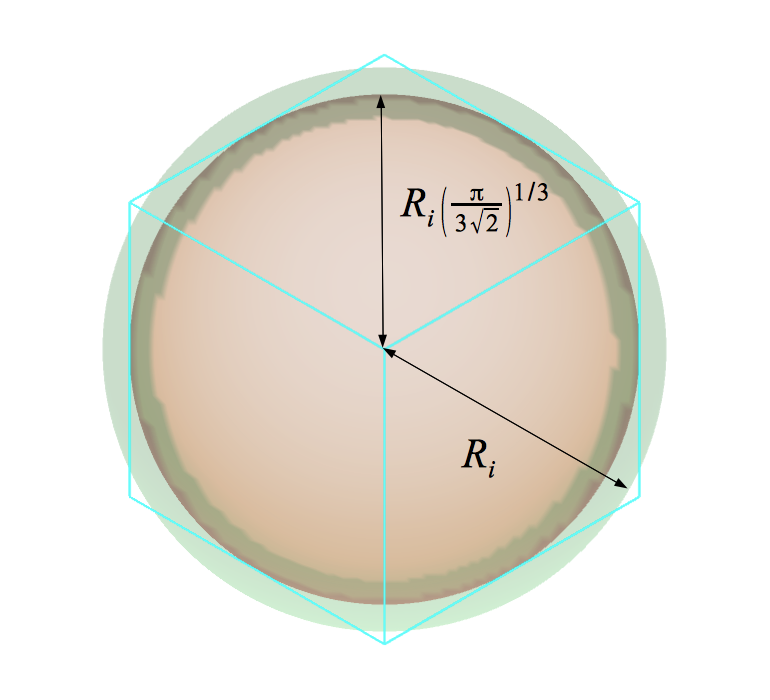
\includegraphics{../../images/MECAGEN/potential/apf_sphere.png}The green sphere has the same volume as the trapezo-rhombic dodecahedron. The pink sphere has a radius $r_{eq} = c_{eq} (R_i+R_j)$, it is tangent to each face of the TDR.

The intrisicness of the notion of equilibrium frees the requirement of the neighbor particles to have the same radius. We apply the equation XX ( $r_{eq} = c_{eq} \left ( R_i + R_j \right )$ ) for every pair of neighbor particles, with no discrimination of size.      ...
\\ ...
\\ ...
\\

\paragraph{3.2.3.1. Attraction-Repulsion  }

As illustrated in figure XX, the attraction/repulsion potential must be repulsive for a distance below $R_{eq}$, attractive between $R_{eq}$ and $R_{max}$ and null afterward.
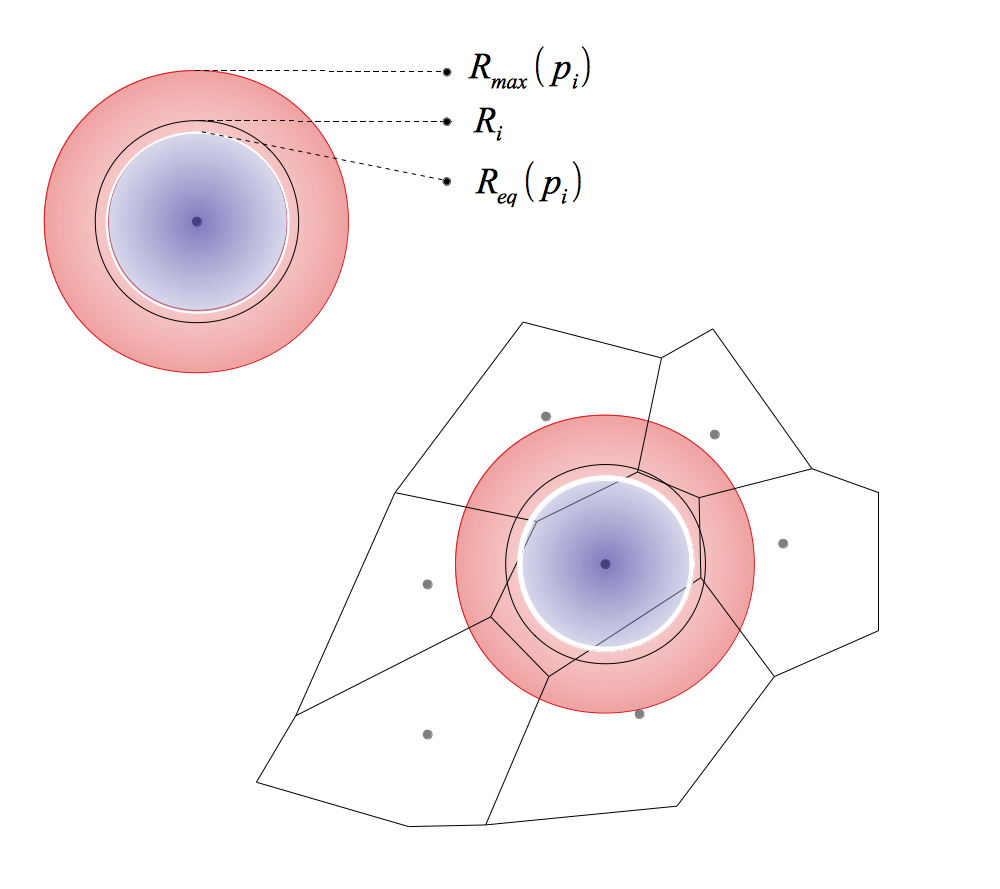
\includegraphics{../../images/MECAGEN/potential/surface_distance_why_potential.png}
\includegraphics{../../images/MECAGEN/potential/surface_distance_why_potential_attr.png}
\includegraphics{../../images/MECAGEN/potential/surface_distance_why_potential_eq.png}
\includegraphics{../../images/MECAGEN/potential/surface_distance_why_potential_rep.png}

We considered the simplest form of potential which catches the short range repulsion / long range attraction property. An spring force derived from the elastic potential.

The mechanical interaction between neighbor cell has been intensively studied by the biophysical scientific communauty. Roughly, the consensual hypothesis is that the driving mechanism is the intercellular surface tension. The two main components of the tension are the adhesion which tends to lower it and the cortical tension which acts antogonistically. The balance between these two components determine the behavior of the interaction: attraction or repulsion. 

Another mechanism is also fundamental: cell preserve their volume. As we made the assumption that cell are spheroidal and that each cellular interaction is decorrelated from the other in its expression, we have to assume that the volume conservation principle participate to the repulsive part of the potential only. This allow us to introduce a discontinuity of the slope of force at the distance of equilibrium. Also, we will denote by adhesion the cumulated effect of effective surface adhesion and cortical tension.

To modulate the intensity of adhesion, we split the stiffness coefficient below and after equilibrium (see $F_{linear}$ figure XX). A low (resp. high) adhesion coefficient $w$ will induce a weak (resp. strong) attraction.
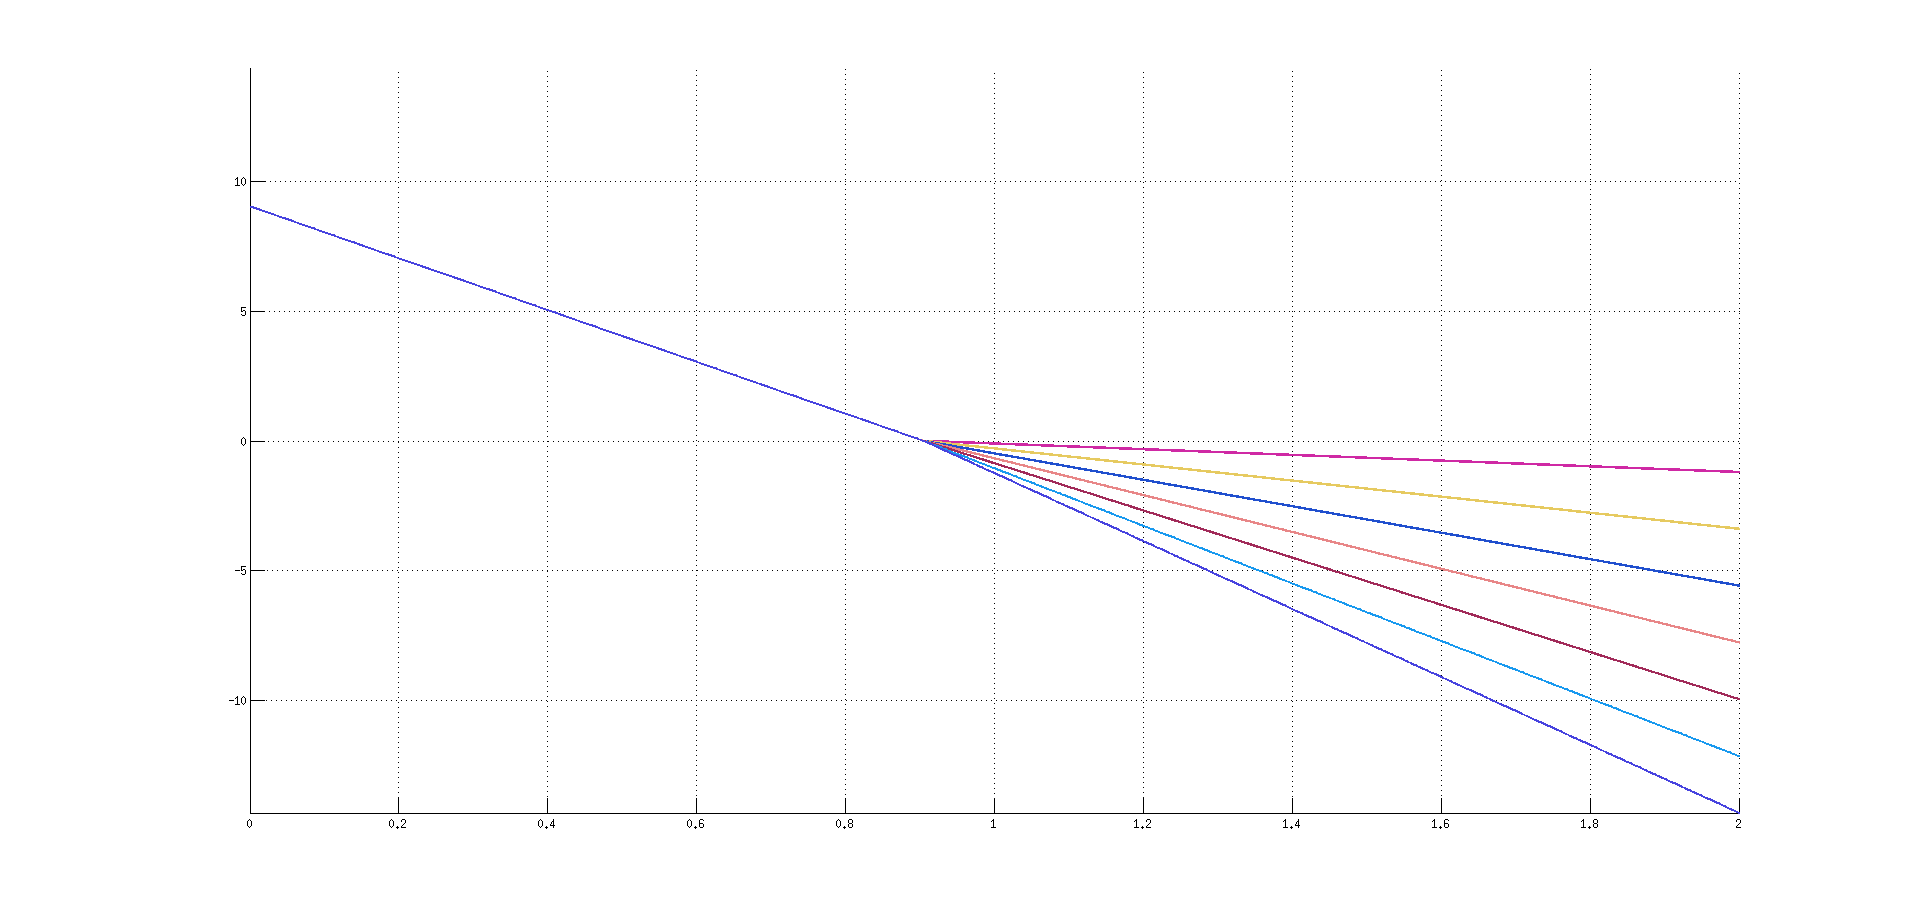
\includegraphics{../../images/MECAGEN/potential/potential_linear_force.png}

$$F_{\text{linear}} = \begin{cases} - rep (r-r_{eq})  & \text{if }r< r_{eq} \\ - w (r-r_{eq}) & \text{if }r\geq r_{eq}  \end{cases}$$

Cells start to adhere when their relative distance is less than $R_{max}$. Moreover, the intensity of the attraction can not be maximum at this point, a bell shape between $R_{eq}$ and $R_{max}$ suits more a realistic cellular interaction.

We obtain this shape by multiplying the linear force $F_{linear}$ by the area of the surface of contact elaborated in X.X.X.X. The depth of the well is still controled by the adhesion coefficient $w$ (see figure XX).
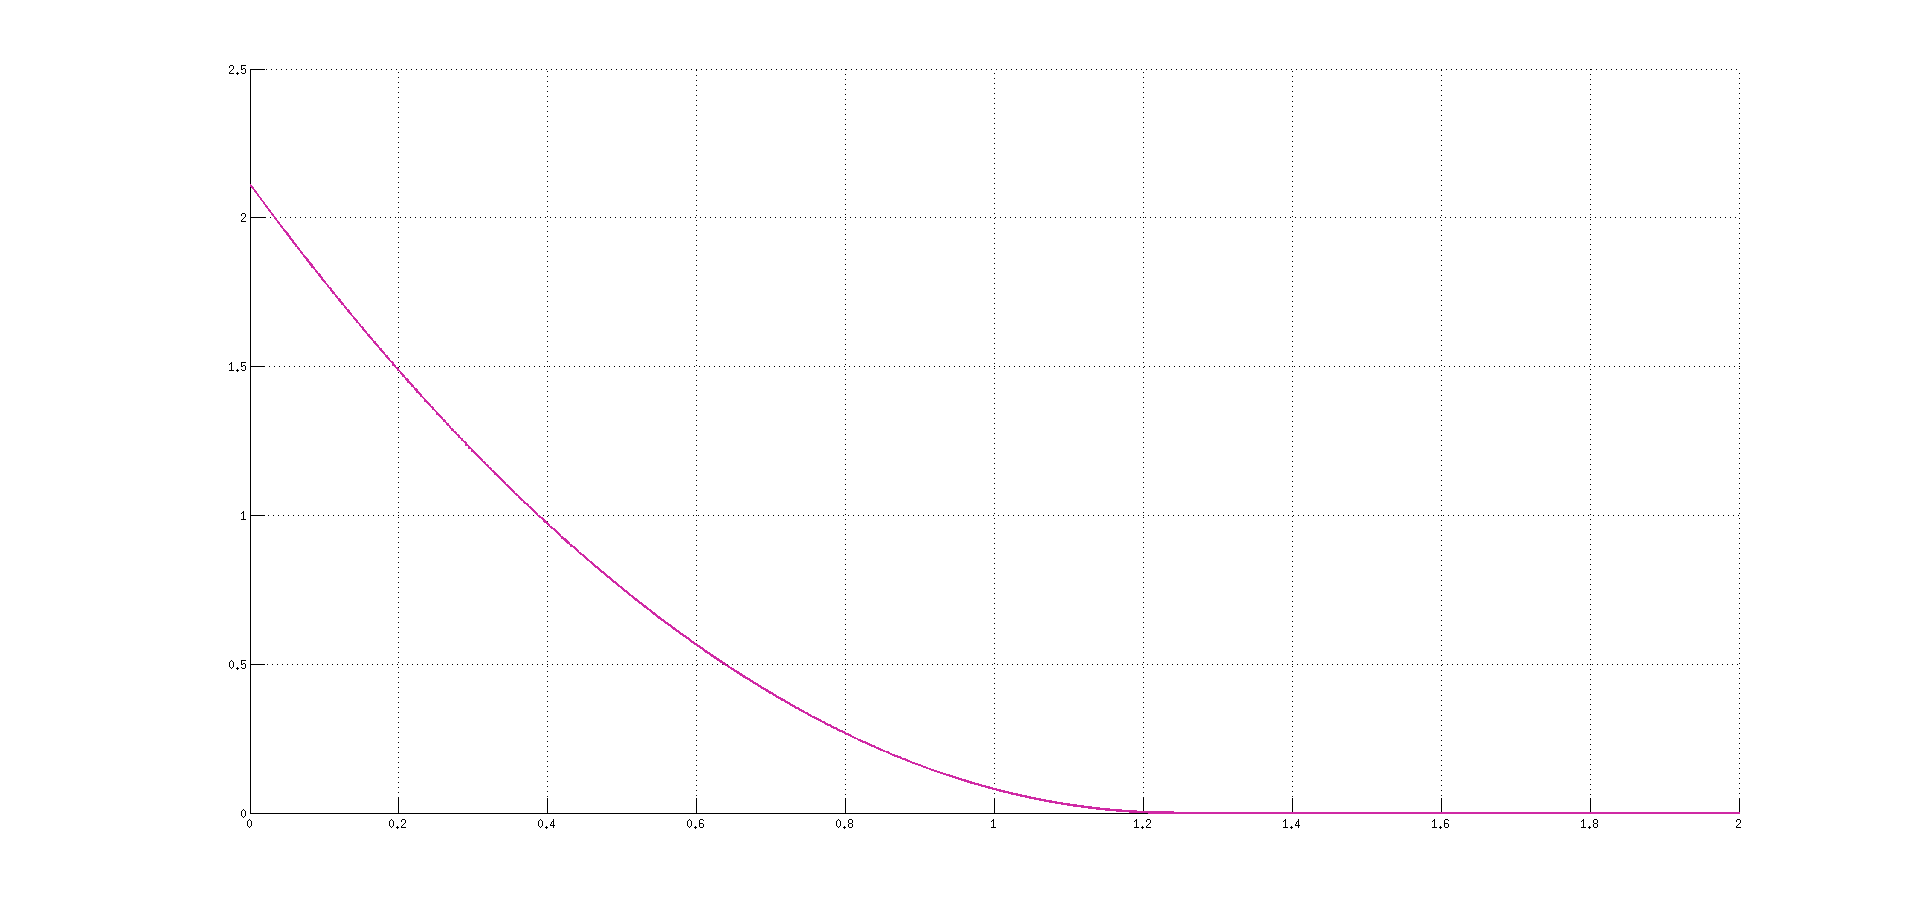
\includegraphics{../../images/MECAGEN/potential/potential_surface.png}

$$A(r,R_i,R_j) = \begin{cases}  a (r - l (R_i+R_j))^2 & \text{if } r < l (R_i+R_j) \\ 0 & \text{if } r \geq l(R_i+R_j)  \end{cases}$$
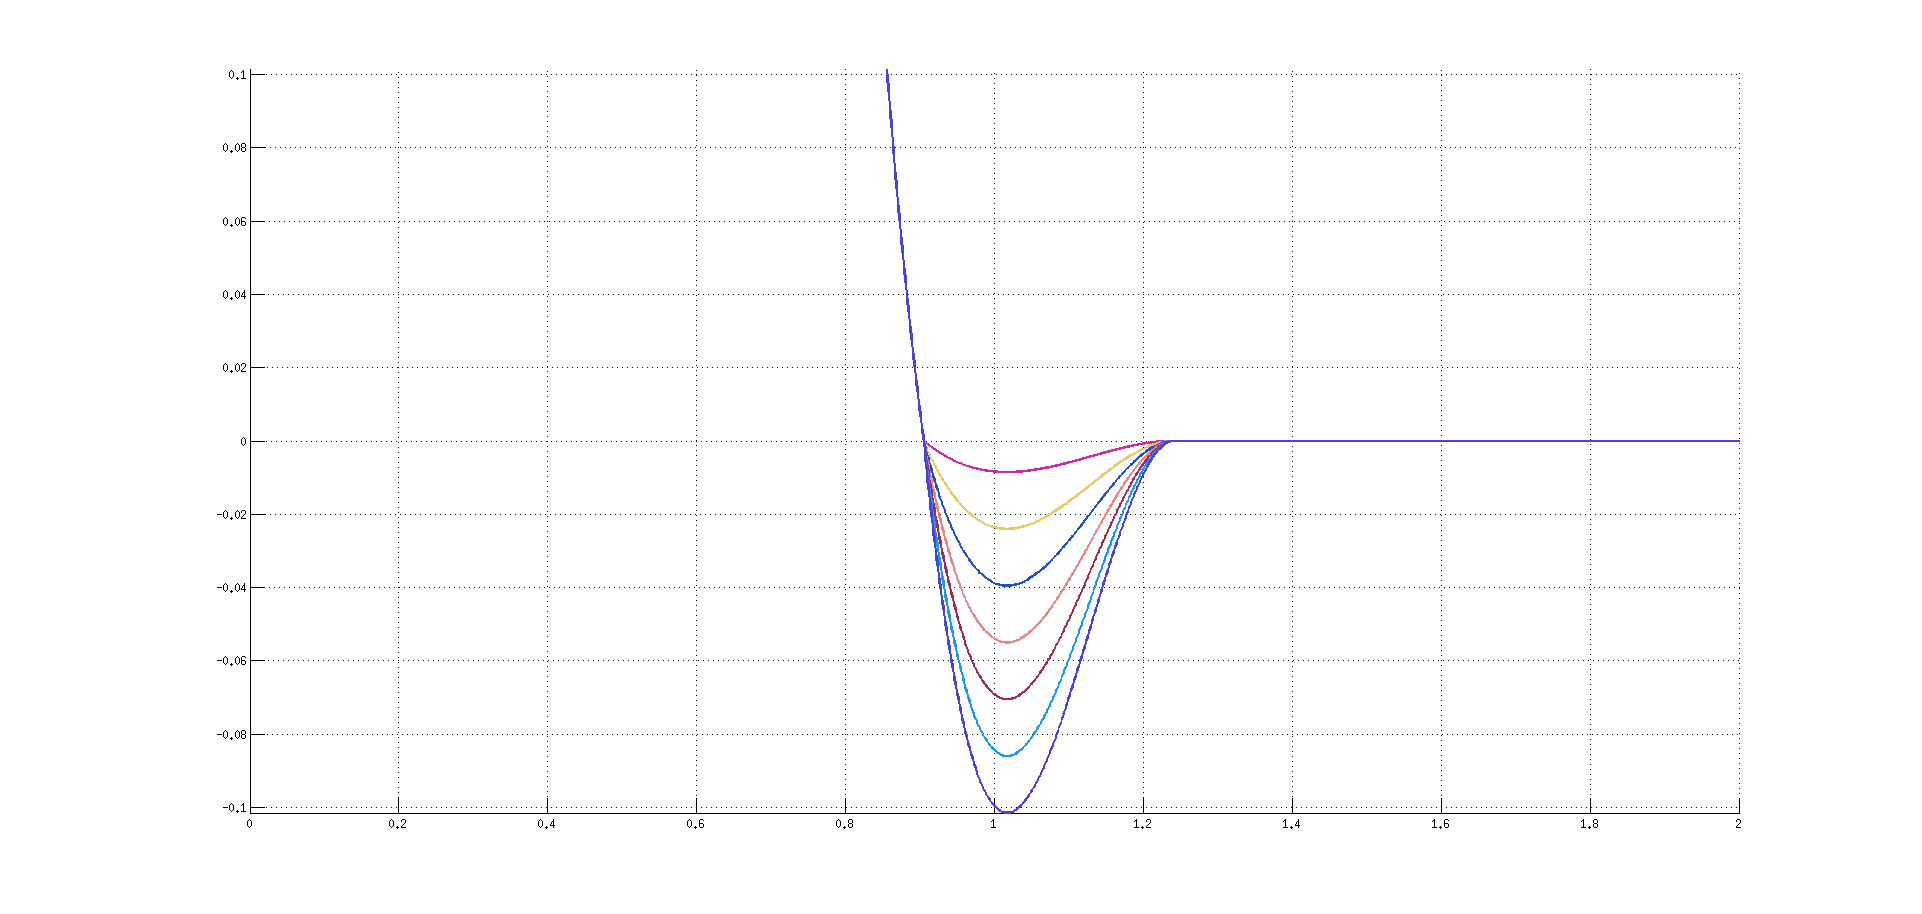
\includegraphics{../../images/MECAGEN/potential/potential_linear_force_scale.png}

$$F = \begin{cases} - rep (r-r_{eq}) \cdot A(r,R_i,R_j)  & \text{if }r< r_{eq} \\ - w (r-r_{eq})  \cdot A(r,R_i,R_j) & \text{if }r\geq r_{eq} \wedge r \leq r_{max} \\ 0 & \text{if } r \geq r_{max}  \end{cases}$$   ...
\\ ...
\\ ...
\\ ...
\\

\paragraph{3.2.3.2. Cell specific behavioral forces  }   ...
\\ ...
\\ ...
\\ ...
\\ ...
\\ ...
\\ ...
\\ ...
\\ ...
\\ ...
\\ ...
\\ ...
\\ ...
\\ ...
\\ ...
\\ ...
\\ ...
\\ ...
\\ ...
\\ ...
\\ ...
\\ ...
\\ ...
\\ ...
\\ ...
\\ ...
\\ ...
\\ ...
\\ ...
\\ ...
\\ ...
\\ ...
\\ ...
\\ ...
\\ ...
\\ ...
\\ ...
\\ ...
\\ ...
\\ ...
\\ ...
\\ ...
\\ ...
\\ ...
\\ ...
\\ ...
\\ ...
\\ ...
\\ ...
\\ ...
\\

\subparagraph{3.2.3.2.1. Protrusion  }

see Weak Law of Action and Reaction for non central forces en.wikibooks.org/wiki/Classical_Mechanics/Newtonian_Physics ...
\\ ...
\\ ...
\\ ...
\\ ...
\\ ...
\\ ...
\\ ...
\\ ...
\\ ...
\\ ...
\\ ...
\\ ...
\\ ...
\\ ...
\\ ...
\\ ...
\\ ...
\\ ...
\\ ...
\\ ...
\\ ...
\\ ...
\\ ...
\\ ...
\\ ...
\\ ...
\\ ...
\\ ...
\\ ...
\\ ...
\\ ...
\\ ...
\\ ...
\\ ...
\\ ...
\\ ...
\\ ...
\\ ...
\\ ...
\\ ...
\\ ...
\\ ...
\\ ...
\\ ...
\\ ...
\\ ...
\\ ...
\\ ...
\\ ...
\\

\subparagraph{3.2.3.2.2. Intercalation-Migration  }   ...
\\ ...
\\ ...
\\ ...
\\ ...
\\ ...
\\ ...
\\ ...
\\ ...
\\ ...
\\ ...
\\ ...
\\ ...
\\ ...
\\ ...
\\ ...
\\ ...
\\ ...
\\ ...
\\ ...
\\ ...
\\ ...
\\ ...
\\ ...
\\ ...
\\ ...
\\ ...
\\ ...
\\ ...
\\ ...
\\ ...
\\ ...
\\ ...
\\ ...
\\ ...
\\ ...
\\ ...
\\ ...
\\ ...
\\ ...
\\ ...
\\ ...
\\ ...
\\ ...
\\ ...
\\ ...
\\ ...
\\ ...
\\ ...
\\ ...
\\

\subsubsection{3.2.4. Zebrafish specificities  }   ...
\\ ...
\\ ...
\\ ...
\\ ...
\\ ...
\\ ...
\\ ...
\\ ...
\\ ...
\\ ...
\\ ...
\\ ...
\\ ...
\\ ...
\\ ...
\\ ...
\\ ...
\\ ...
\\ ...
\\ ...
\\ ...
\\ ...
\\ ...
\\ ...
\\ ...
\\ ...
\\ ...
\\ ...
\\ ...
\\ ...
\\ ...
\\ ...
\\ ...
\\ ...
\\ ...
\\ ...
\\ ...
\\ ...
\\ ...
\\ ...
\\ ...
\\ ...
\\ ...
\\ ...
\\ ...
\\ ...
\\ ...
\\ ...
\\ ...
\\

\subsection{3.3. Discussion  }   ...
\\ ...
\\ ...
\\ ...
\\ ...
\\ ...
\\ ...
\\ ...
\\ ...
\\ ...
\\ ...
\\ ...
\\ ...
\\ ...
\\ ...
\\ ...
\\ ...
\\ ...
\\ ...
\\ ...
\\ ...
\\ ...
\\ ...
\\ ...
\\ ...
\\ ...
\\ ...
\\ ...
\\ ...
\\ ...
\\ ...
\\ ...
\\ ...
\\ ...
\\ ...
\\ ...
\\ ...
\\ ...
\\ ...
\\ ...
\\ ...
\\ ...
\\ ...
\\ ...
\\ ...
\\ ...
\\ ...
\\ ...
\\ ...
\\ ...
\\

\subsubsection{3.3.1. Alternative-Future work including previous experiments  }   ...
\\ ...
\\ ...
\\ ...
\\ ...
\\ ...
\\ ...
\\ ...
\\ ...
\\ ...
\\ ...
\\ ...
\\ ...
\\ ...
\\ ...
\\ ...
\\ ...
\\ ...
\\ ...
\\ ...
\\ ...
\\ ...
\\ ...
\\ ...
\\ ...
\\ ...
\\ ...
\\ ...
\\ ...
\\ ...
\\ ...
\\ ...
\\ ...
\\ ...
\\ ...
\\ ...
\\ ...
\\ ...
\\ ...
\\ ...
\\ ...
\\ ...
\\ ...
\\ ...
\\ ...
\\ ...
\\ ...
\\ ...
\\ ...
\\ ...
\\

\subsubsection{3.3.2. Extracellular matrix  }   ...
\\ ...
\\ ...
\\ ...
\\ ...
\\ ...
\\ ...
\\ ...
\\ ...
\\ ...
\\ ...
\\ ...
\\ ...
\\ ...
\\ ...
\\ ...
\\ ...
\\ ...
\\ ...
\\ ...
\\ ...
\\ ...
\\ ...
\\ ...
\\ ...
\\ ...
\\ ...
\\ ...
\\ ...
\\ ...
\\ ...
\\ ...
\\ ...
\\ ...
\\ ...
\\ ...
\\ ...
\\ ...
\\ ...
\\ ...
\\ ...
\\ ...
\\ ...
\\ ...
\\ ...
\\ ...
\\ ...
\\ ...
\\ ...
\\ ...
\\

\subsubsection{3.3.3. Friction  }   ...
\\ ...
\\ ...
\\ ...
\\ ...
\\ ...
\\ ...
\\ ...
\\ ...
\\ ...
\\ ...
\\ ...
\\ ...
\\ ...
\\ ...
\\ ...
\\ ...
\\ ...
\\ ...
\\ ...
\\ ...
\\ ...
\\ ...
\\ ...
\\ ...
\\ ...
\\ ...
\\ ...
\\ ...
\\ ...
\\ ...
\\ ...
\\ ...
\\ ...
\\ ...
\\ ...
\\ ...
\\ ...
\\ ...
\\ ...
\\ ...
\\ ...
\\ ...
\\ ...
\\ ...
\\ ...
\\ ...
\\ ...
\\ ...
\\ ...
\\